\documentclass[11pt,a4paper]{article}
\usepackage[margin=20mm]{geometry}
\usepackage{fontspec}
\setmainfont{DejaVu Serif}
\setsansfont{DejaVu Sans}
\setmonofont{DejaVu Sans Mono}[Scale=0.85]
\usepackage{polyglossia}
\setdefaultlanguage{russian}
\usepackage{graphicx}
\usepackage{hyperref}
\usepackage{enumitem}
\usepackage{fancyvrb}
\hypersetup{hidelinks}
\setlength{\parindent}{0pt}
\setlength{\parskip}{4pt}
\usepackage{titlesec}
\titleformat{\section}{\large\bfseries}{}{0pt}{}
\titlespacing*{\section}{0pt}{10pt}{4pt}
\sloppy
\setlist{nosep,leftmargin=*}
\emergencystretch=3em
\newcommand{\shot}[2]{\begin{center}\includegraphics[width=\linewidth,height=.34\textheight,keepaspectratio]{#1}\par\small #2\end{center}}
\begin{document}
\begin{center}
{\small Университет ИТМО · Фронт-энд разработка · 2026}\par
{\LARGE Лабораторная работа № 1}\par
{\large Статический интерфейс ML-платформы}\par
Светлов Ярослав, группа J3211
\end{center}
\section*{Цель и исходные материалы}
Создать интерфейс платформы управления ML-экспериментами на HTML, CSS и JavaScript. Использована существующая работа из PR-ветки pr-198 (совпадает с веткой lab1), без исправлений кода при подготовке отчёта. Вариант 2.
\section*{Реализация}
\begin{itemize}
\item Формы входа и регистрации, личный кабинет, навигационное меню.
\item Поиск по демонстрационным экспериментам и вывод таблицы результатов.
\item Экран деталей с графиком Chart.js, метриками, логами и артефактами.
\item Разметка в index.html, стили в style.css, данные и обработчики в script.js. Bootstrap и внешние библиотеки загружаются из CDN.
\end{itemize}

\section*{Проверка и выявленные ограничения}
Проверка проведена 19.09.2026 в Firefox 148.0.2 и Chromium 146.0.7680.153. Работают переходы между экранами, обязательные поля формы, фильтрация, пустая выдача и вкладки деталей.\begin{itemize}
\item Ошибка выбора: поиск ResNet показывает ResNet-50-Base, но кнопка открытия всегда ведёт к статическим деталям BERT-Transformer-v2. ID эксперимента не передаётся.
\item На ширине 390 px открытое меню сжимает содержимое; ширина документа достигает 487 px. В свёрнутом меню обрезается кнопка выхода.
\item Управление моделью и деплой остаются заглушками. Артефакты представлены текстом без скачивания.
\item Вход имитируется сменой экрана. Настоящей авторизации, API и сохранения сессии в этой статической работе нет.
\end{itemize}

\section*{Запуск}
Из папки \texttt{labs/lab1}:
\begin{verbatim}
python3 -m http.server 3001 --bind 127.0.0.1
\end{verbatim}
Открыть \url{http://localhost:3001}. Для CDN нужен интернет. Сервер останавливается сочетанием Ctrl+C.
\section*{Вывод}
Основные экраны статического прототипа присутствуют. Работа не считается полностью проверенной без замечаний: требуется исправить выбор эксперимента и мобильную вёрстку. Заглушки отделены от реализованного функционала.

\clearpage
\section*{Скриншоты}
\shot{checks/lab1-dashboard.png}{Рисунок 1. Личный кабинет статического прототипа.}
\shot{checks/lab1-wrong-experiment.png}{Рисунок 2. После выбора ResNet показан BERT: зафиксированная ошибка.}

\clearpage
\section*{Скриншоты (продолжение)}
\begin{center}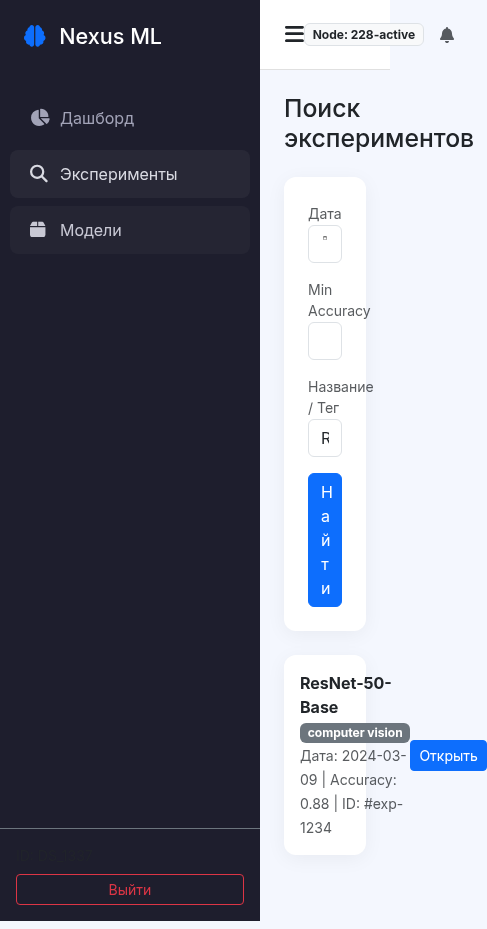
\includegraphics[height=.7\textheight,keepaspectratio]{checks/chromium-lab1-390-expanded.png}\par\small Рисунок 3. Проблема компоновки при ширине окна 390 px.\end{center}

\end{document}
